\documentclass[12pt, a4paper]{article}
\usepackage{amsmath}
\usepackage{amsfonts}
\usepackage{amsthm}
\usepackage{mathtools}
\newtheorem{theorem}{Theorem}[section]
\newtheorem{definition}{Definition}[section]
\numberwithin{equation}{section}
\usepackage{pgfplots}
\pgfplotsset{width=10cm,compat=1.9}
\graphicspath{ {img/} }
\DeclareGraphicsExtensions{.png}

\title{Restricted Boltzmann Machines}
\author{Kristian Wichmann}

\begin{document}
\maketitle

\section{Boltzmann machines}
A \textit{Boltzmann machine} is a collection of units divided into two parts: A \textit{visible layer} and a \textit{hidden layer}. The \textit{state} of unit $i$ is represented by a number $s_i$. According to the type of machine considered, these may take one different ranges of values. All units are connected to every other unit, with \textit{weights} $w_{ij}$ being the connection between units $i$ and $j$. Figure \ref{fig:bm} shows an example of such a atructure. In addition, unit $i$ has a \textit{bias} $\theta_i$.

\begin{figure}
\centering
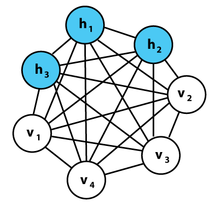
\includegraphics{bm}
\caption{The structure of a general Boltzmann machine with 4 visible and 3 hidden units.}
\label{fig:bm}
\end{figure}

The \textit{energy} of the machine is:
\begin{equation}
E=-\left(\sum_{i<j}w_{ij}s_i s_j+\sum_i\theta_i s_i\right)
\end{equation}


\section{Restricted Boltmann machines}
A \textit{restricted Boltzmann machine} (RBM) is a Boltzmann machine where there's no connections between units in the two layers. Assuming there's $n$ visible, and $m$ hidden units, this means that we may write the energy:
\begin{equation}
E=-\left(\sum_{i=1}^n a_i v_i+\sum_{j=1}^m b_j h_j+\sum_{i=1}^n\sum_{j=1}^m v_i w_{ij}h_j\right)
\end{equation}

\begin{figure}
\centering
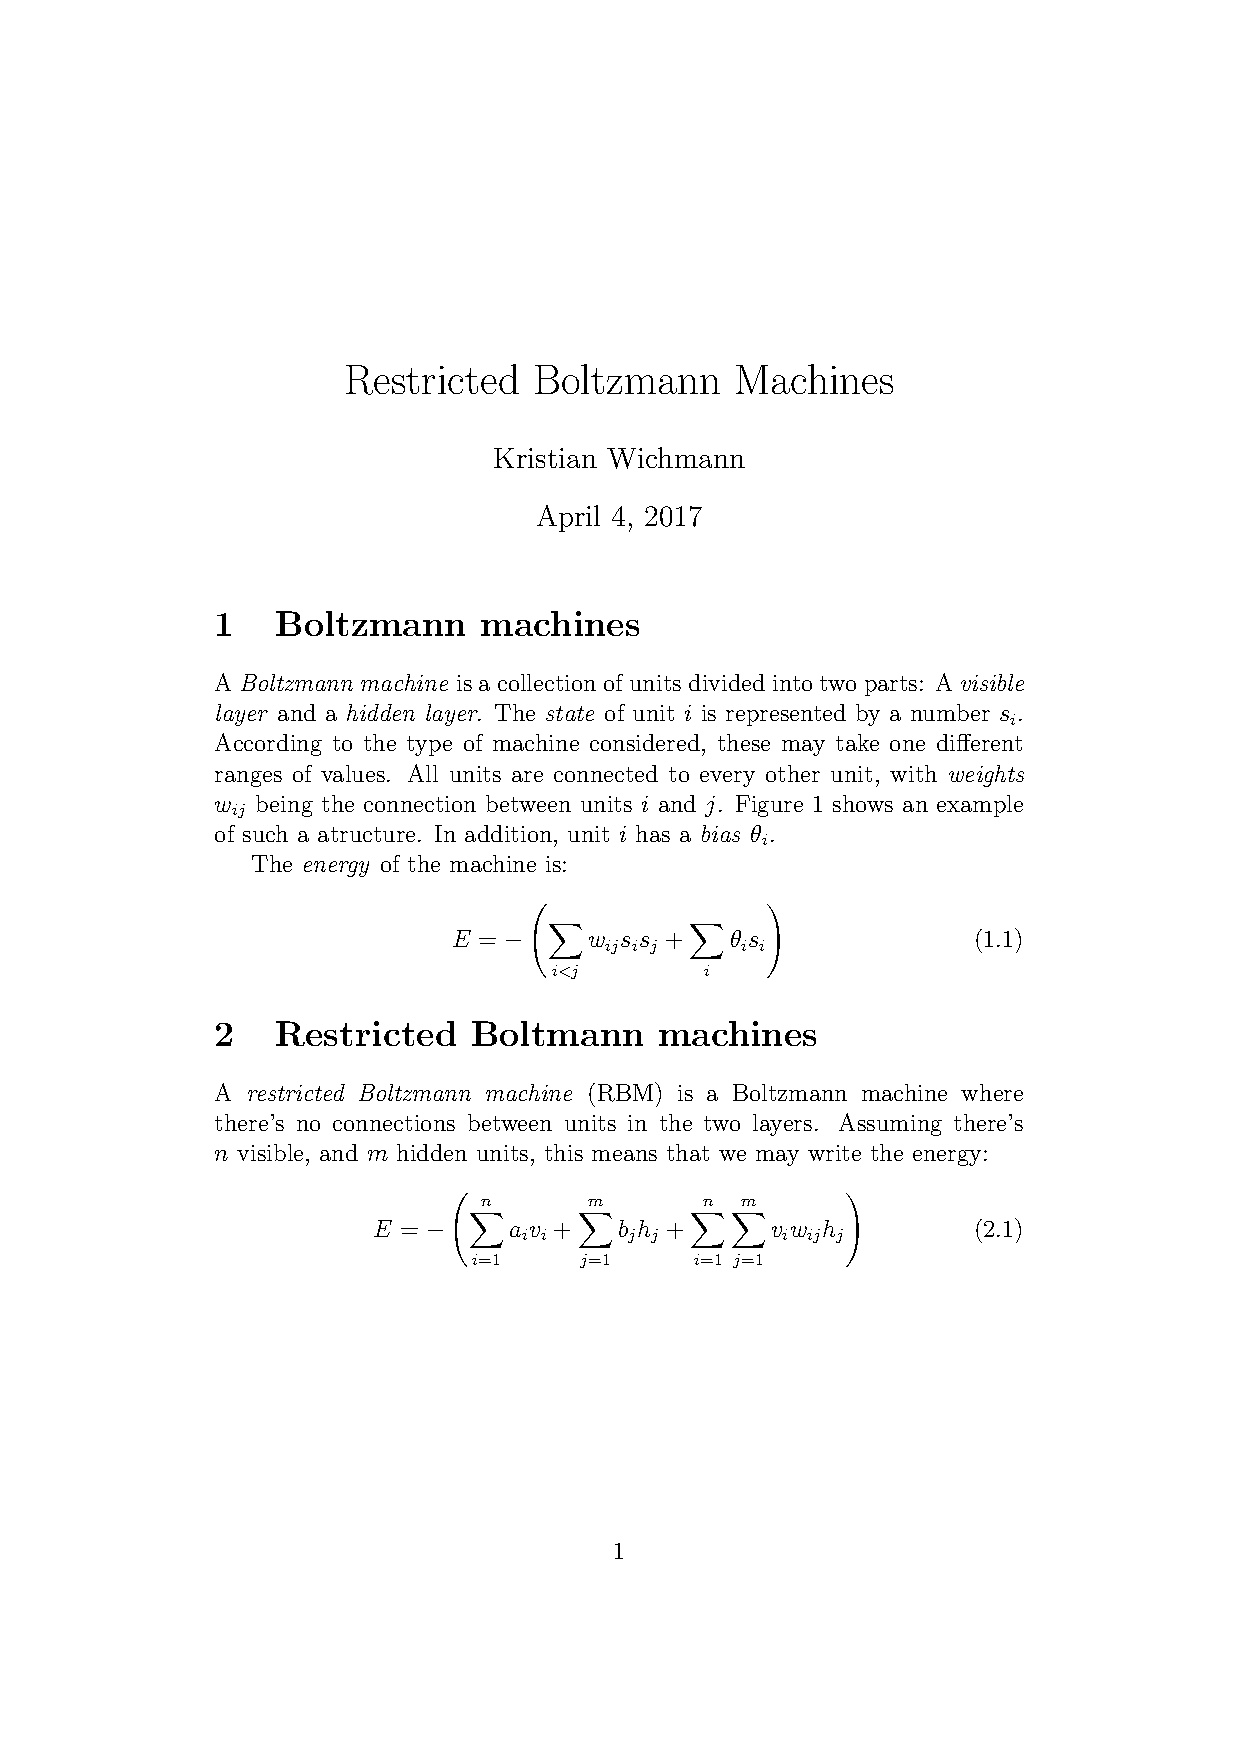
\includegraphics{rbm}
\caption{The structure of a restricted Boltzmann machine with 3 visible and 4 hidden units.}
\label{fig:rbm}
\end{figure}

\end{document}